%=========================================================================
% sec-tune
%=========================================================================

\section{Tuning the Floyd-Warshall Algorithm}
\label{sec-tune}

\subsection{Copy Optimization}
\label{sec-tune-copy}

We implemented copy optimization to address the cache locality issue
raised by the VTune profiler. At the beginning of each iteration of the
function square, we create an additional transposed copy of the matrix,
so that we can use this matrix when accessing the array in row-major
order. We can see significant performance gains from doing so, especially
as the number of nodes in the graph increases as shown in
Figure~\ref{fig-tune-copy-0}.

\begin{figure}[h]
  \centering
  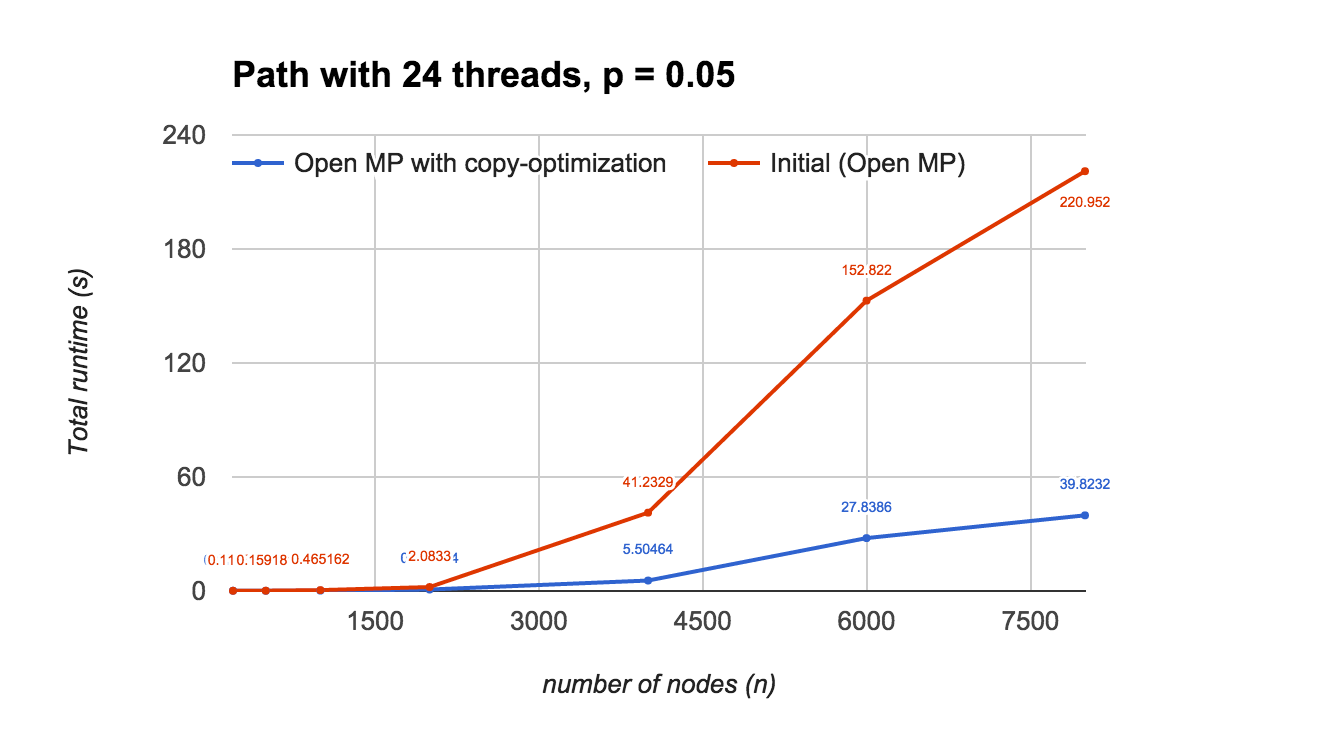
\includegraphics[width=0.8\tw]{fig-tune-copy-0.png}
  \caption{\textbf{Performance of Copy Optimization --} Execution time of
    the parallel implementation of the algorithm running with 24 threads
    across a wide range of dataset sizes with and without copy
    optimization.}
  \label{fig-tune-copy-0}
\end{figure}

From this experiment, we can see that when n is small (< 1000), the
overheads from copying outweighs the benefits of cache locality, but as
the number of nodes increases past 1000, we see significant improvement
gains.

\begin{figure}[h]
  \centering
  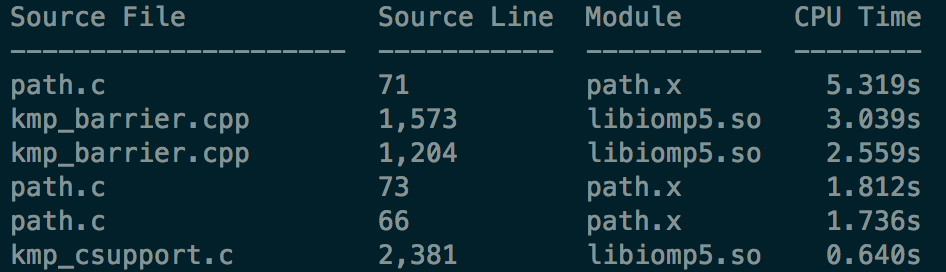
\includegraphics[width=0.8\tw]{fig-tune-copy-1.png}
  \caption{\textbf{VTune profiling output of Open MP with copy/transpose
      optimization}}
  \label{fig-tune-copy-1}
\end{figure}

The performance benefits of reading from a transposed copy of the matrix
is also shown in the profiling output of the tuned code in
Figure~\ref{fig-tune-copy-1}, as seen from the reduced CPU time.

\subsection{Manual Vectorization}
\label{sec-tune-vector}

In order to best utilize the resources on both the compute nodes and the
accelerator device, it is critical to ensure that the code we execute is
properly vectorized. Although modern compilers are capable of
auto-vectorizing code, the results can be inconsistent and often requires
the user to massage the code in such a way that the compiler can
recognize opportunities for vectorization. As such, manually vectorizing
code using intrinsics is commonly used when optimizing performance
critical kernels, such as the \texttt{square()} function in the
Floyd-Warshall algorithm for this assignment.

%=========================================================================
% fig-tune-vector.tex
%=========================================================================

\begin{figure}[h]

  \centering
  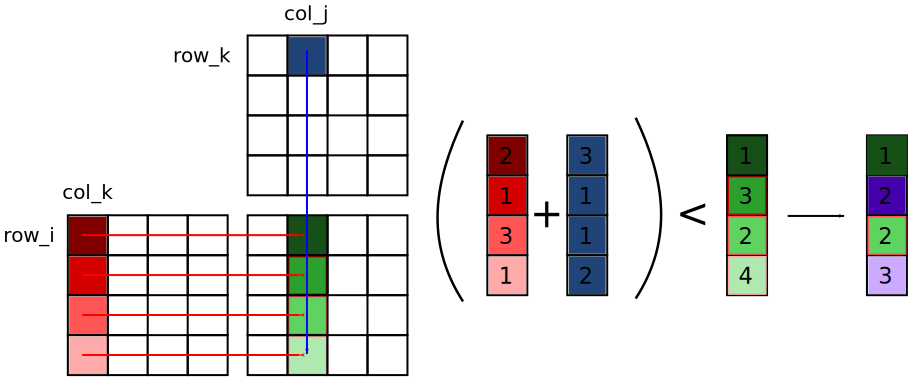
\includegraphics[width=0.9\tw]{fig-tune-vector.svg.pdf}

  \caption{\textbf{Overview of Manual Vectorization Strategy --} All
    matrices shown on the left side represent the same shortest path
    matrix. The elements of the k-th column are added to the (k,j)-th
    element and compared against the current shortest path value in the
    (i,j)-th element. An example vectorized computation with a vector
    length of 4 is shown on the right, where the final result to be
    stored only contains the elements with the shortest paths between the
    sum vector and the current vector. }

  \label{fig-tune-vector}

\end{figure}


The vectorization strategy used here is similar to that used in matrix
multiplication; the difference is that we are operating on a single
matrix and we need to do a comparison instead of a multiplication. The
primary insight here is that all elements in the k-th column need to be
added the same element in the k-th row of the j-th column, where
the (i,j)-th element is the output being calculated (i.e., the shortest
path between node i and j). Therefore, we vectorize the computation for
calculating a vector length worth of outputs in the j-th column as shown
in Figure~\ref{fig-tune-vector}.

Using manual vectorization, we can vector load the elements in both the
j-th and k-th columns, and broadcast the (k,j)-th element to a vector
register. Although vector loads/stores to non-vector-aligned addresses are
allowed, such unaligned or masked operations are much less efficient
than the aligned variants. This becomes relevant when the number of nodes
(i.e., the dimension of the matrix) is not evenly divisible by the vector
length. In this case, even if we force the alignment of per-core local
buffers, none of the columns after the first are guaranteed to be
aligned. We address this by over-allocating the local buffers with extra
padding elements so that each column is always a multiple of the vector
length. The \texttt{pack\_padded\_data()} and
\texttt{unpack\_padded\_data()} functions are used to copy columns
between the unaligned local buffer to the aligned local buffer so that
each column starts at a vector-aligned address. The overhead of this copy
is captured in the timing loop.

The most challenging aspect of vectorization in this algorithm is
actually the comparison. We use a vector greater-than comparison that can
be used to check if the (i,k) to (k,j) path (i.e., the sum vector) is
less than the current shortest path in (i,j) (i.e., the current
vector). This returns a vector with an enabled mask (0xffffffff) for
elements that had a true comparison, or a disabled mask (0x00000000) for
elements that had a false comparison. If any of the elements in the mask
vector are 1s, we know that computation is not yet done and we need to
clear the done variable. We can do this with a vector testc operation
that returns true only if the mask vector is all 0s. In order to
determine the output elements, we first AND the mask vector with the sum
vector to zero-out the elements that were not shorter than the current
shortest path. Conversely, we AND the NOT of the mask vector with the
current vector to zero-out the elements that are not the shortest path
anymore. By adding these masked vectors, we obtain a vector of the newest
shortest paths that we can vector store to the j-th column.

If the matrix dimensions are not evenly divisible by the vector length,
the mask vector must also be further masked to zero-out the elements that
correspond to junk beyond the padding elements when computing the last
iteration for a given column.

Experiments show that using manual vectorization achieves a ~75\% speedup
compared to using only auto-vectorization on the parallel implementation
of the Floyd-Warshall algorithm running on the compute nodes.
